\chapter{Implementation}


\section{Initialization}
People usually oversimplify data integration by assuming it involves only extract, transform and load (ETL) tools. Though critical, an ETL tool is just one piece of a complex puzzle.
The data integration framework (DIF) encompasses two categories of processes. Before transforming our data into information that businesspeople can use to analyze and make decisions, we need to start by gathering our data physically from its sources and preparing our metadata.
\vskip0.2cm
Thus, we start our project by establishing our databases connection, whether input resources or output destinations. 
\vskip0.2cm
Figure \ref{fig:ssmsDB} shows our initial database in local sql server
\begin{figure}[H]
\centering
\frame{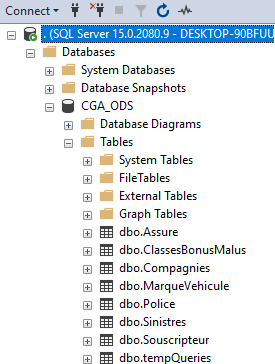
\includegraphics[width=0.5\columnwidth]{img/Implementation/Initialization/ssmsDB.PNG}}
\caption{sql server database}
\label{fig:ssmsDB}
\end{figure}
\vskip0.2cm

\clearpage
Figure \ref{fig:csvDB} shows our csv files for more data
\begin{figure}[H]
\centering
\frame{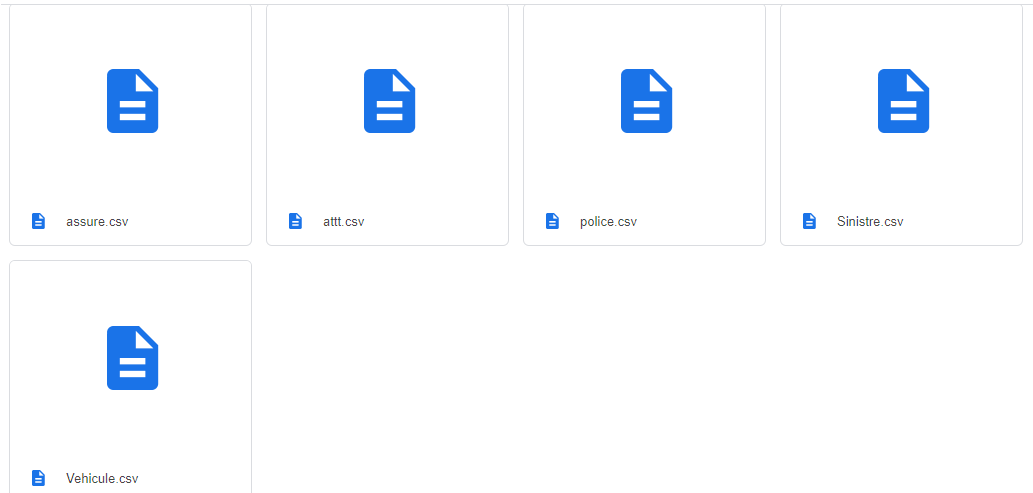
\includegraphics[width=0.5\columnwidth]{img/Implementation/Initialization/csvDB.PNG}}
\caption{csv files}
\label{fig:csvDB}
\end{figure}

\vskip0.2cm
As in Figure \ref{fig:psqlDB} we created our exporting database in PostgreSQL
\begin{figure}[H]
\centering
\frame{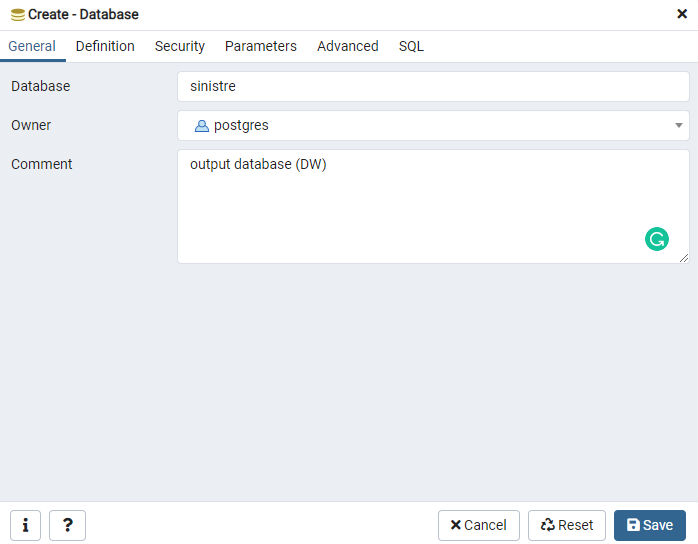
\includegraphics[width=0.5\columnwidth]{img/Implementation/Initialization/psqlDB.PNG}}
\caption{PostgreSQL database created}
\label{fig:psqlDB}
\end{figure}
\vskip0.2cm

We need to connect to multiple databases, then we want to centralize the connection information details in the Metadata folder in the Repository tree view as given in figure\ref{fig:metadata}.
\begin{figure}[H]
\centering
\frame{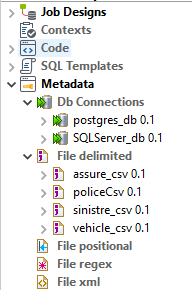
\includegraphics[width=0.3\columnwidth]{img/Implementation/Initialization/metadata.PNG}}
\caption{Talend Metadata}
\label{fig:metadata}
\end{figure}
\vskip0.2cm

This setup procedure is made of two separate but closely related major tasks:
\vskip0.2cm

\quad\quad\quad 1- Set up our database connections,

\quad\quad\quad 2- Retrieve the tables schemas.

\quad\quad\quad 3- Set up our delmitied csv files.

1- As shown in Figures \ref{fig:sqlConec} and \ref{fig:psqlConec}  we configured our database connections
\begin{figure}[H]
\centering
\frame{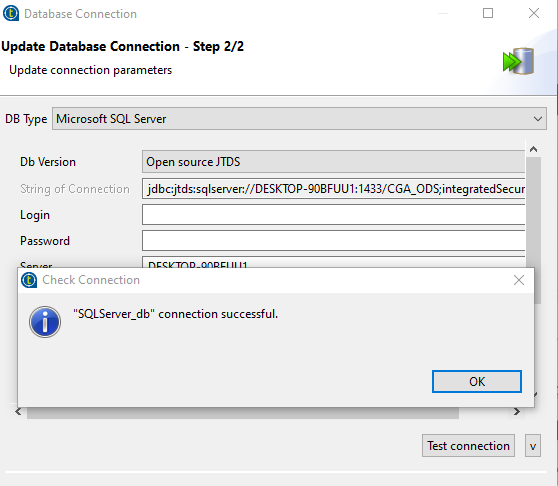
\includegraphics[width=0.5\columnwidth]{img/Implementation/Initialization/sqlConec.PNG}}
\caption{Microsoft sql server DB connection}
\label{fig:sqlConec}
\end{figure}

\begin{figure}[H]
\centering
\frame{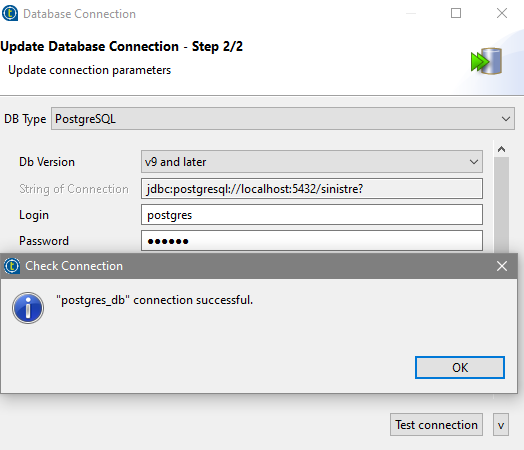
\includegraphics[width=0.5\columnwidth]{img/Implementation/Initialization/psqlConec.PNG}}
\caption{PostgreSQL DB connection}
\label{fig:psqlConec}
\end{figure}
\vskip0.2cm
\clearpage
2- To retrieve table schemas from the database connection you have just set up, right-click the connection item from the Repository tree view, and select Retrieve schema from the contextual menu.Then we simply follow the wizards.

\begin{figure}[H]
\centering
\frame{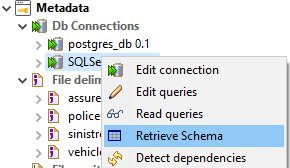
\includegraphics[width=0.5\columnwidth]{img/Implementation/Initialization/schemas.PNG}}
\caption{retrieving schemas}
\label{fig:psqlConec}
\end{figure}

3- We finally import our csv files by following the delimited files wizards

\begin{figure}[H]
\centering
\frame{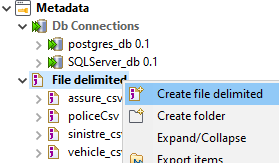
\includegraphics[width=0.5\columnwidth]{img/Implementation/Initialization/filedelimited.PNG}}
\caption{importing csv files}
\label{fig:psqlConec}
\end{figure}
\clearpage
\section{Data Integration with Talend}
    % Une sous section
    \subsection{Table : Assure}
To implement our first table "Assure", we start by setting up our input component, Microsoft SQL server Database. We define the needed table, its schema ... etc.
\begin{figure}[H]
\centering
\frame{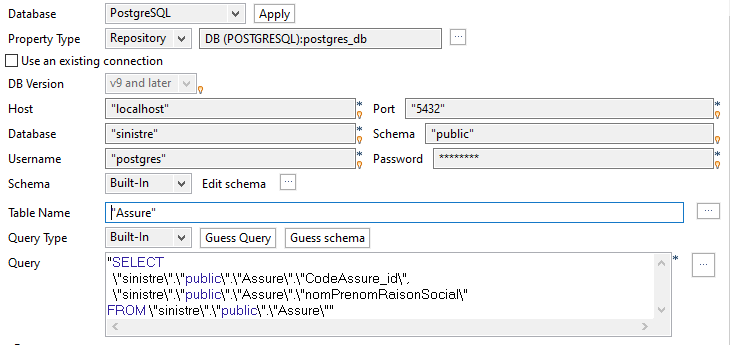
\includegraphics[width=0.8\columnwidth]{img/Implementation/talend/assure/0.PNG}}
\end{figure}
\vskip0.2cm
        
Then, we set up our data importing job, to import all rows from MS SQL to our output database PSQL
\begin{figure}[H]
\centering
\frame{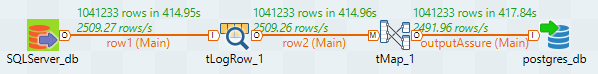
\includegraphics[width=0.8\columnwidth]{img/Implementation/talend/assure/1.0.PNG}}
\end{figure}
\vskip0.2cm
\begin{figure}[H]
\centering
\frame{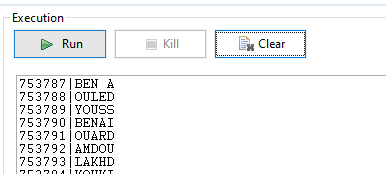
\includegraphics[width=0.8\columnwidth]{img/Implementation/talend/assure/1.1.PNG}}
\end{figure}
\vskip0.2cm
\clearpage

Next, we explore our Assure.csv file where we notice we have 2 new columns that we need to include. 
\begin{figure}[H]
\centering
\frame{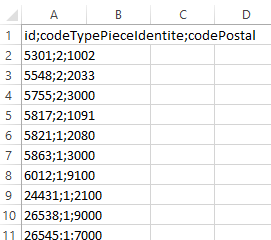
\includegraphics[width=0.4\columnwidth]{img/Implementation/talend/assure/1.2.PNG}}
\end{figure}
\vskip0.2cm

We setup our components to merge the csv data, we do that by using TMap, configured as following 
\begin{figure}[H]
\centering
\frame{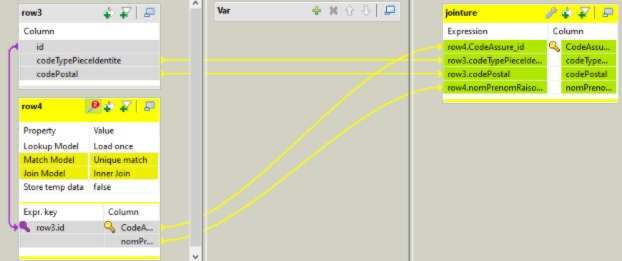
\includegraphics[width=0.8\columnwidth]{img/Implementation/talend/assure/1.3.0.PNG}}
\end{figure}
\vskip0.2cm

An expected error occured, which is about not finding the 2 new columns in the PSQL Assure table.
\begin{figure}[H]
\centering
\frame{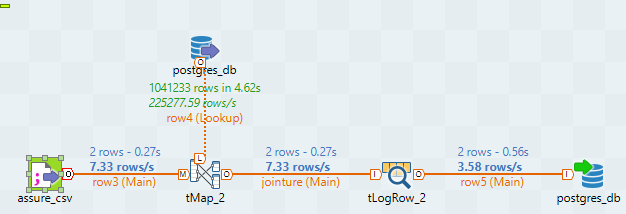
\includegraphics[width=0.8\columnwidth]{img/Implementation/talend/assure/1.3.PNG}}
\end{figure}
\vskip0.2cm
\begin{figure}[H]
\centering
\frame{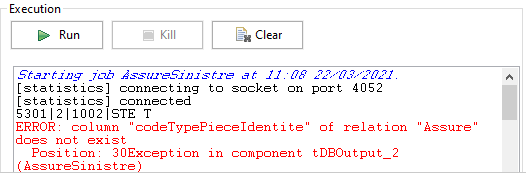
\includegraphics[width=0.8\columnwidth]{img/Implementation/talend/assure/1.4.PNG}}
\end{figure}
\vskip0.2cm

We fix that by manually creating the new columns
\begin{figure}[H]
\centering
\frame{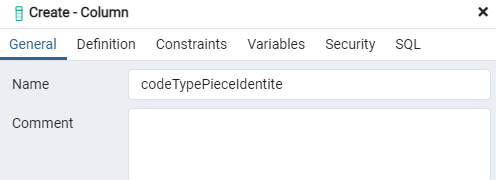
\includegraphics[width=0.8\columnwidth]{img/Implementation/talend/assure/1.5.PNG}}
\end{figure}
\vskip0.2cm

Then as seen in the next we figure the job should be done correctly : we update 12795 out or 25934 rows from MS SQL with new columns from csv file 
\begin{figure}[H]
\centering
\frame{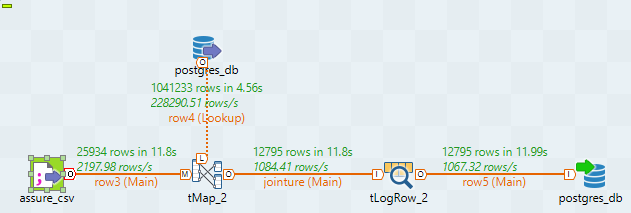
\includegraphics[width=0.8\columnwidth]{img/Implementation/talend/assure/1.6.PNG}}
\end{figure}
\vskip0.2cm

Even though the exportation is completed we notice these errors in TLog, which implies that we have some outliers to fix in our data.
\begin{figure}[H]
\centering
\frame{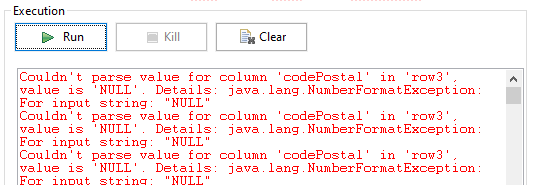
\includegraphics[width=0.8\columnwidth]{img/Implementation/talend/assure/1.7.PNG}}
\end{figure}
\vskip0.2cm

Now we add the remaining data from our csv. 
\begin{figure}[H]
\centering
\frame{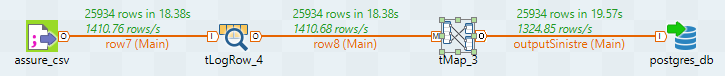
\includegraphics[width=0.8\columnwidth]{img/Implementation/talend/assure/1.8.PNG}}
\end{figure}

The outliers errors are shown again in csv data
\begin{figure}[H]
\centering
\frame{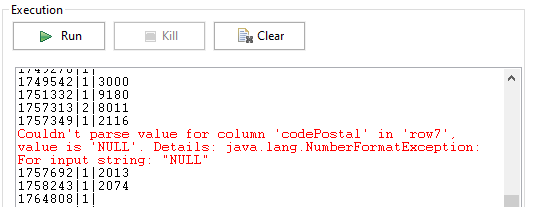
\includegraphics[width=0.8\columnwidth]{img/Implementation/talend/assure/1.9.PNG}}
\end{figure}

Our data is ready to explore in PSQL
\begin{figure}[H]
\centering
\frame{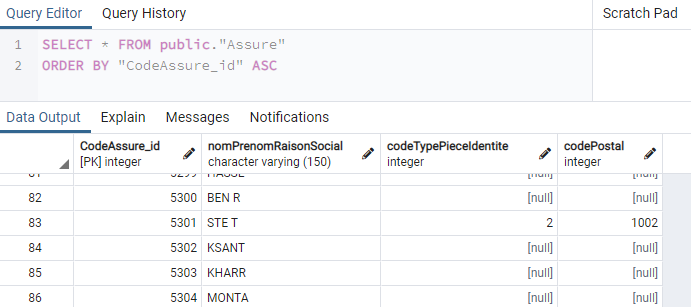
\includegraphics[width=0.8\columnwidth]{img/Implementation/talend/assure/1.10.PNG}}
\end{figure}

We noticed a lot of NULL values, which is completely normal since the csv files updated only 25000 files while our initial database from MS SQL had more than 1M rows 
\begin{figure}[H]
\centering
\frame{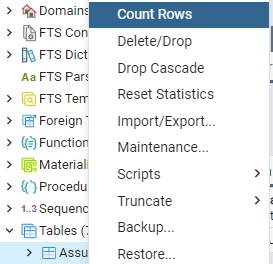
\includegraphics[width=0.4\columnwidth]{img/Implementation/talend/assure/1.11.PNG}}
\end{figure}
\begin{figure}[H]
\centering
\frame{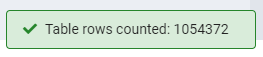
\includegraphics[width=0.4\columnwidth]{img/Implementation/talend/assure/1.12.PNG}}
\end{figure}

To fix that we start inspecting our first column to see how many NULL values does it contain. 
\begin{figure}[H]
\centering
\frame{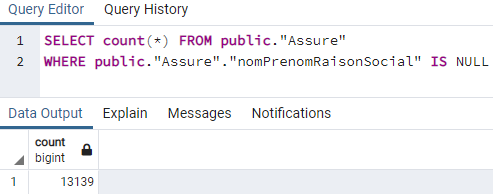
\includegraphics[width=0.7\columnwidth]{img/Implementation/talend/assure/1.13.PNG}}
\end{figure}


In first column "NomPrenomRaisonSocial" we have 13139, we can generate random values for that column using this sql query 
\begin{figure}[H]
\centering
\frame{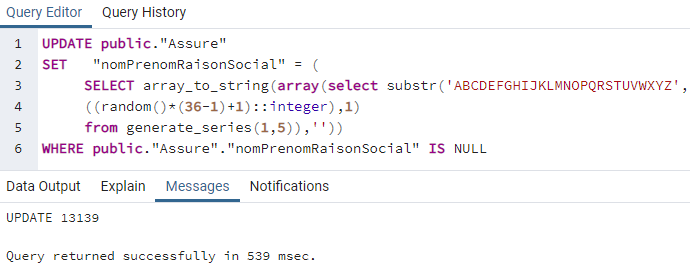
\includegraphics[width=0.8\columnwidth]{img/Implementation/talend/assure/1.15.PNG}}
\end{figure}

The second column to inspect is "CodeTypePieceIdentite" which has a lot of null values
\begin{figure}[H]
\centering
\frame{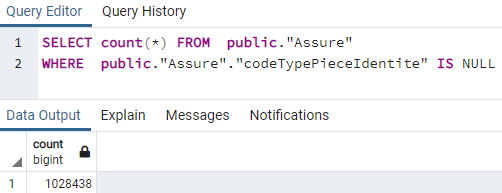
\includegraphics[width=0.8\columnwidth]{img/Implementation/talend/assure/1.16.PNG}}
\end{figure}

\clearpage

from exploring the data we noticed that "CodeTypePieceIdentite" column should be containing either "1" or "2" as values, so we can replace those null values using this update with a subselect generator,
\begin{figure}[H]
\centering
\frame{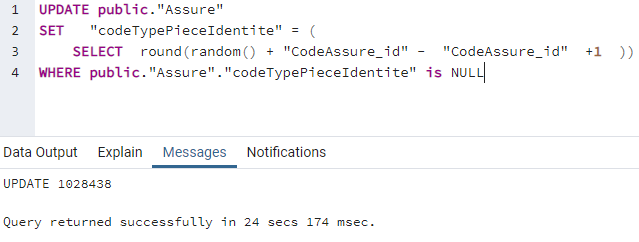
\includegraphics[width=0.8\columnwidth]{img/Implementation/talend/assure/1.18.PNG}}
\end{figure}

This is what we get
\begin{figure}[H]
\centering
\frame{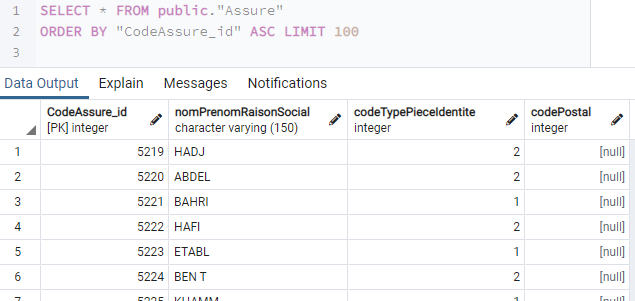
\includegraphics[width=0.8\columnwidth]{img/Implementation/talend/assure/1.19.PNG}}
\end{figure}

We can do that differently using the TRowGenerator
\begin{figure}[H]
\centering
\frame{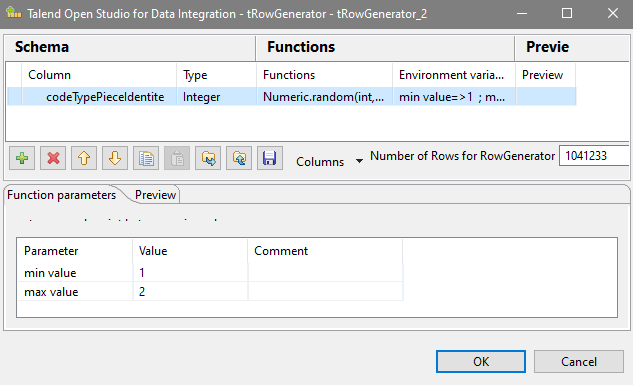
\includegraphics[width=0.8\columnwidth]{img/Implementation/talend/assure/1.21.PNG}}
\end{figure}
\begin{figure}[H]
\centering
\frame{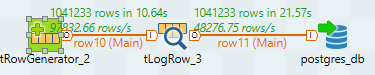
\includegraphics[width=0.4\columnwidth]{img/Implementation/talend/assure/1.20.PNG}}
\end{figure}

The last column to inspect is "CodePostal", which contains also a lot of null variable, at first we didn't want to randomly generate values for this column because that can critically affect or analysis.
\vskip0.2cm 
So we tried this query to retrieve randomly from NON-NULL existing values to complete the missing data
\begin{figure}[H]
\centering
\frame{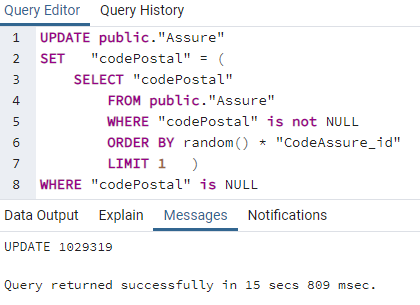
\includegraphics[width=0.8\columnwidth]{img/Implementation/talend/assure/1.22.PNG}}
\end{figure}

This query couldn't do the job so we tried to optimize it, we tried first to use CTE
\begin{figure}[H]
\centering
\frame{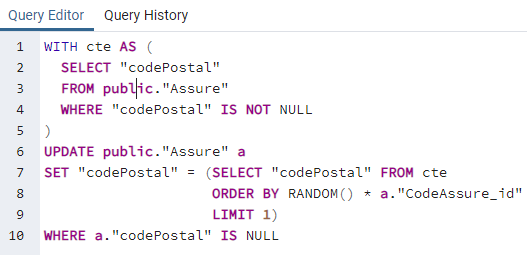
\includegraphics[width=0.8\columnwidth]{img/Implementation/talend/assure/1.24.PNG}}
\end{figure}

Also we tried to use window functions as following
\begin{figure}[H]
\centering
\frame{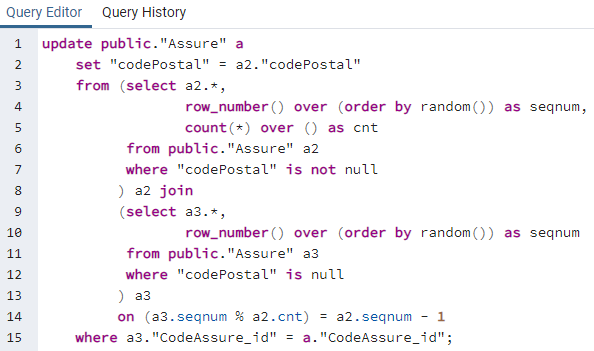
\includegraphics[width=0.8\columnwidth]{img/Implementation/talend/assure/1.25.PNG}}
\end{figure}

All 3 tries stuck in executing and never do the job, even though we confirm that all 3 queries work perfectly for smaller dataset,  we concluded that this fail is probably due to large data size table. 
\vskip0.2cm
As alternative solution we decided to use the following query to generate the missing values
\begin{figure}[H]
\centering
\frame{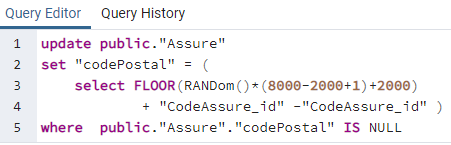
\includegraphics[width=0.8\columnwidth]{img/Implementation/talend/assure/1.26.PNG}}
\end{figure}

This is the final ressult
\begin{figure}[H]
\centering
\frame{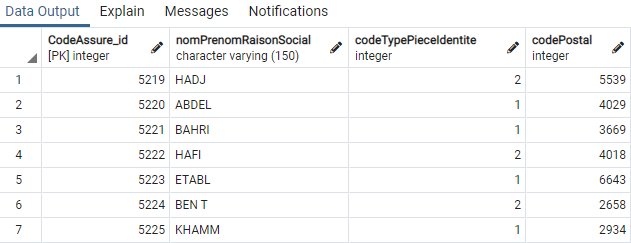
\includegraphics[width=0.8\columnwidth]{img/Implementation/talend/assure/1.27.PNG}}
\end{figure}



%%%%%%%%%%%%%%%%%%%%%%%%%%%%%%%%%%%%%%%%%%%%%%%%%%%%%%%%%%%%%%%%%%%%%%%%%
\subsection{Table : Police}
We start by exploring our data in SSMS.
\begin{figure}[H]
\centering
\frame{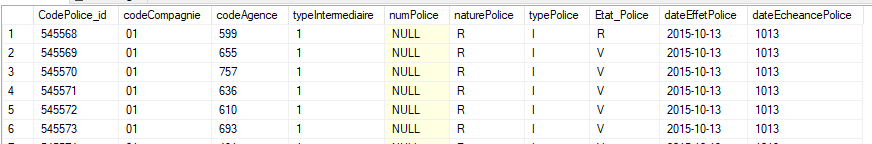
\includegraphics[width=0.8\columnwidth]{img/Implementation/talend/assure/2.2.PNG}}
\end{figure}

A null column is noticed, we exclude that from our TMapping 
\begin{figure}[H]
\centering
\frame{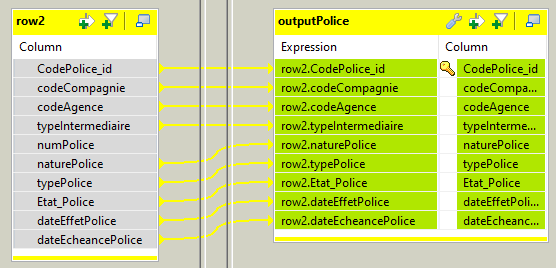
\includegraphics[width=0.8\columnwidth]{img/Implementation/talend/assure/2.3.PNG}}
\end{figure}

No new useful data in csv file.
\begin{figure}[H]
\centering
\frame{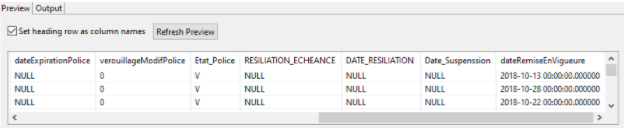
\includegraphics[width=0.8\columnwidth]{img/Implementation/talend/assure/2.4.PNG}}
\end{figure}

So we simply run the following job:
\begin{figure}[H]
\centering
\frame{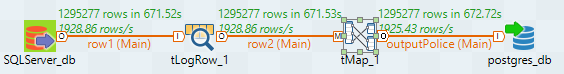
\includegraphics[width=0.8\columnwidth]{img/Implementation/talend/assure/2.0.PNG}}
\end{figure}

\subsection{Table : Vehicule, MarqueVehicule, UsageVehicule }

From SSMS we noticed 2 null columns, we remvoe that from out TMap component
\begin{figure}[H]
\centering
\frame{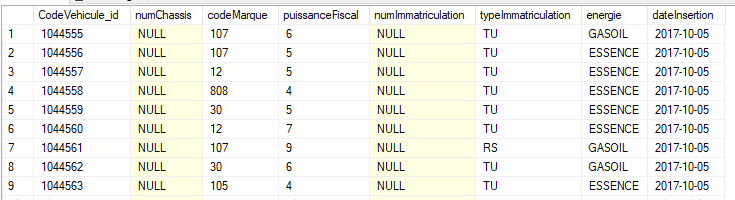
\includegraphics[width=0.8\columnwidth]{img/Implementation/talend/assure/3.0.PNG}}
\end{figure}

Then run the job to import data from MS SQL to PSQL
\begin{figure}[H]
\centering
\frame{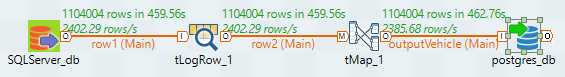
\includegraphics[width=0.8\columnwidth]{img/Implementation/talend/assure/3.1.PNG}}
\end{figure}

Using same components but different configurations, we can import table "UsageVehicule"
\begin{figure}[H]
\centering
\frame{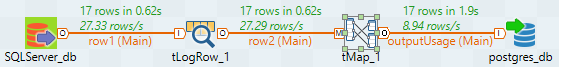
\includegraphics[width=0.8\columnwidth]{img/Implementation/talend/assure/3.3.0.PNG}}
\end{figure}

And "MarqueVehicule" Table
\begin{figure}[H]
\centering
\frame{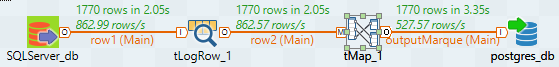
\includegraphics[width=0.8\columnwidth]{img/Implementation/talend/assure/3.3.PNG}}
\end{figure}

"CodeUsage" column is missed from "Vehicule" Table, we can fix that by : first, creating the column manually
\begin{figure}[H]
\centering
\frame{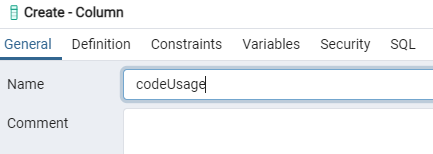
\includegraphics[width=0.8\columnwidth]{img/Implementation/talend/assure/3.4.PNG}}
\end{figure}

Second, we can use the next query to randomly select values from "UsageVehicule" and fill the new column
\begin{figure}[H]
\centering
\frame{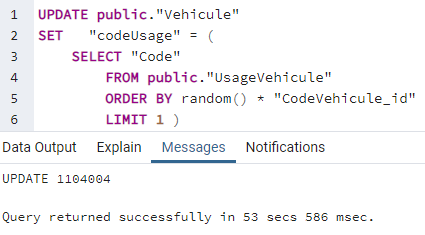
\includegraphics[width=0.8\columnwidth]{img/Implementation/talend/assure/3.5.PNG}}
\end{figure}

This is our final Vehicule table ready to be used
\begin{figure}[H]
\centering
\frame{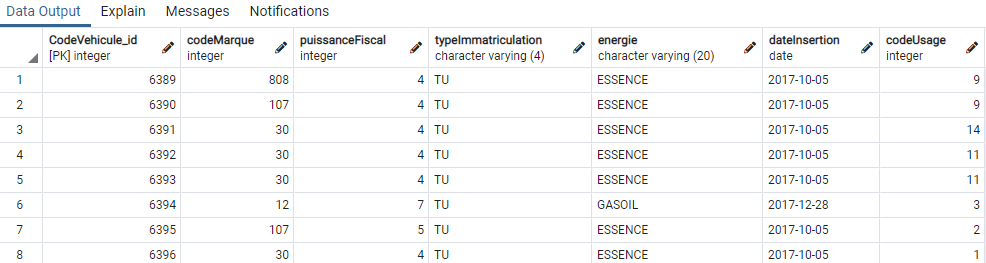
\includegraphics[width=0.8\columnwidth]{img/Implementation/talend/assure/3.6.PNG}}
\end{figure}


\subsection{Table : Sinistre}
Most of our data is in our csv file, so we start by merging our data sources in TMap component, to ADD the in common rows
\begin{figure}[H]
\centering
\frame{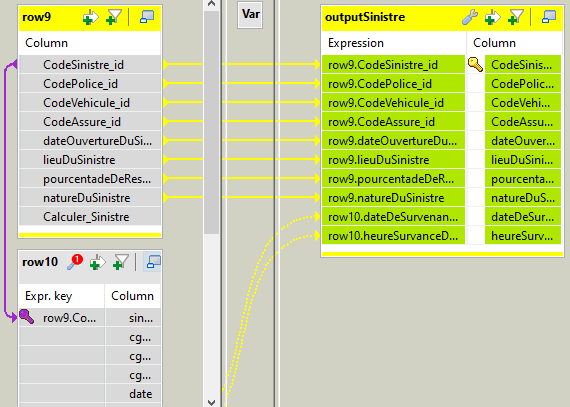
\includegraphics[width=0.8\columnwidth]{img/Implementation/talend/assure/7.0.PNG}}
\end{figure}
\begin{figure}[H]
\centering
\frame{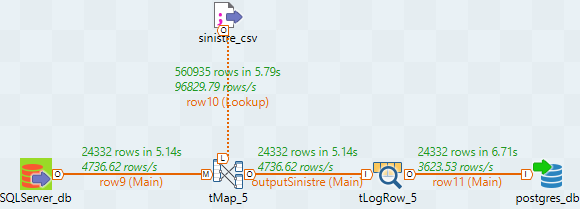
\includegraphics[width=0.8\columnwidth]{img/Implementation/talend/assure/7.1.PNG}}
\end{figure}
\begin{figure}[H]
\centering
\frame{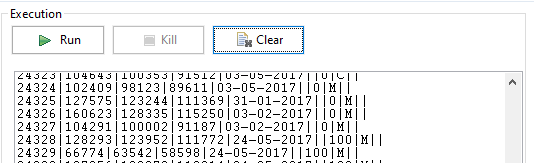
\includegraphics[width=0.8\columnwidth]{img/Implementation/talend/assure/7.2.PNG}}
\end{figure}

Then we add the remaning data from our csv file to PSQL table
\begin{figure}[H]
\centering
\frame{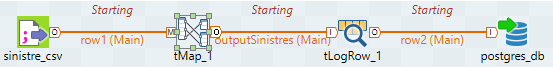
\includegraphics[width=0.8\columnwidth]{img/Implementation/talend/assure/7.3.PNG}}
\end{figure}

We get this error due to date formatting issues,
\begin{figure}[H]
\centering
\frame{\includegraphics[width=0.8\columnwidth]{img/Implementation/talend/assure/7.4.PNG}}
\end{figure}

We can easily pass that error by configuring the column Date Pattern in TMap
\begin{figure}[H]
\centering
\frame{\includegraphics[width=0.8\columnwidth]{img/Implementation/talend/assure/7.5.PNG}}
\end{figure}

Exporting the final table in PSQL
\begin{figure}[H]
\centering
\frame{\includegraphics[width=0.8\columnwidth]{img/Implementation/talend/assure/7.6.PNG}}
\end{figure}

\subsection{Tables : ClassesBonusMalus, souscripteur, companies, typeinfo}

The remaining table were completely ready to be directly exported to PostgreSQL 

\begin{figure}[H]
\centering
\frame{\includegraphics[width=0.8\columnwidth]{img/Implementation/talend/assure/5.PNG}}
\end{figure}



\clearpage
\section{Data Integration with Python}
\subsection{Table: Assure}

We start by creating a new dataframe from our MS SQL table.
\begin{figure}[H]
\centering
\frame{\includegraphics[width=0.8\columnwidth]{img/Implementation/python/1.1.PNG}}
\end{figure}
\begin{figure}[H]
\centering
\frame{\includegraphics[width=0.8\columnwidth]{img/Implementation/python/1.2.PNG}}
\end{figure}

We also import our assure.csv file to a new dataframe.
\begin{figure}[H]
\centering
\frame{\includegraphics[width=0.8\columnwidth]{img/Implementation/python/1.3.PNG}}
\end{figure}
\begin{figure}[H]
\centering
\frame{\includegraphics[width=0.8\columnwidth]{img/Implementation/python/1.4.PNG}}
\end{figure}

Merging both dataframes to one is executed using the following code: 
\begin{figure}[H]
\centering
\frame{\includegraphics[width=0.8\columnwidth]{img/Implementation/python/1.5.PNG}}
\end{figure}
\begin{figure}[H]
\centering
\frame{\includegraphics[width=0.8\columnwidth]{img/Implementation/python/1.6.PNG}}
\end{figure}

Replace NaN values from 'nomPrenomRaisonSocial' column with random strings of 5 characters
\begin{figure}[H]
\centering
\frame{\includegraphics[width=0.8\columnwidth]{img/Implementation/python/1.7.PNG}}
\end{figure}

Replace NaN values from 'codeTypePieceIdentite' column with either 1 or 2 randomly
\begin{figure}[H]
\centering
\frame{\includegraphics[width=0.8\columnwidth]{img/Implementation/python/1.8.PNG}}
\end{figure}

This is what we get after previous transformation
\begin{figure}[H]
\centering
\frame{\includegraphics[width=0.8\columnwidth]{img/Implementation/python/1.9.PNG}}
\end{figure}

Make a list of values from 'codePostal' and use it to randomly fill NaN fields
\begin{figure}[H]
\centering
\frame{\includegraphics[width=0.8\columnwidth]{img/Implementation/python/1.10.PNG}}
\end{figure}
\begin{figure}[H]
\centering
\frame{\includegraphics[width=0.8\columnwidth]{img/Implementation/python/1.11.PNG}}
\end{figure}
\begin{figure}[H]
\centering
\frame{\includegraphics[width=0.8\columnwidth]{img/Implementation/python/1.12.PNG}}
\end{figure}

Change dataframe columns types and push it to PostgreSQL table )
\begin{figure}[H]
\centering
\frame{\includegraphics[width=0.8\columnwidth]{img/Implementation/python/1.13.PNG}}
\end{figure}

This is what we get in PSQL
\begin{figure}[H]
\centering
\frame{\includegraphics[width=0.8\columnwidth]{img/Implementation/python/1.14.PNG}}
\end{figure}

We need to specify the primarykey manualy to remove to read only constraint
\begin{figure}[H]
\centering
\frame{\includegraphics[width=0.8\columnwidth]{img/Implementation/python/1.15.PNG}}
\end{figure}

Or we can do it in PSQL
\begin{figure}[H]
\centering
\frame{\includegraphics[width=0.8\columnwidth]{img/Implementation/python/1.16.PNG}}
\end{figure}

This is our final table in PSQL
\begin{figure}[H]
\centering
\frame{\includegraphics[width=0.8\columnwidth]{img/Implementation/python/1.17.PNG}}
\end{figure}

\subsection{Table: Police}

Create dataframe of Table Police from MS SQL data
\begin{figure}[H]
\centering
\frame{\includegraphics[width=0.8\columnwidth]{img/Implementation/python/2.0.PNG}}
\end{figure}
\begin{figure}[H]
\centering
\frame{\includegraphics[width=0.8\columnwidth]{img/Implementation/python/2.1.PNG}}
\end{figure}

Delete the NULL column 'numPolice' also delete 'dateEcheancePolice' because it gives same data as 'dateEffetPolice'
\begin{figure}[H]
\centering
\frame{\includegraphics[width=0.8\columnwidth]{img/Implementation/python/2.2.PNG}}
\end{figure}

Verify column types and export to PSQL
\begin{figure}[H]
\centering
\frame{\includegraphics[width=0.8\columnwidth]{img/Implementation/python/2.4.PNG}}
\end{figure}

\subsection{Table: Vehicule, MarqueVehicule,UsageVehicule}


Import table 'vehicule'
\begin{figure}[H]
\centering
\frame{\includegraphics[width=0.8\columnwidth]{img/Implementation/python/3.0.PNG}}
\end{figure}

Delete useless Columns
\begin{figure}[H]
\centering
\frame{\includegraphics[width=0.8\columnwidth]{img/Implementation/python/3.1.PNG}}
\end{figure}

Import table 'MarqueVehicule'
\begin{figure}[H]
\centering
\frame{\includegraphics[width=0.8\columnwidth]{img/Implementation/python/3.3.PNG}}
\end{figure}

Import table 'UsageVehicule'
\begin{figure}[H]
\centering
\frame{\includegraphics[width=0.8\columnwidth]{img/Implementation/python/3.4.PNG}}
\end{figure}

'codeUsage' is missed from 'vehicule', we notice that 'codeUsage' is in a range of (1,17), so we can generate the needed it data randomly and add it to the missing fields
\begin{figure}[H]
\centering
\frame{\includegraphics[width=0.8\columnwidth]{img/Implementation/python/3.5.PNG}}
\end{figure}

Finally,persist our tables to PostgreSQL server
\begin{figure}[H]
\centering
\frame{\includegraphics[width=0.8\columnwidth]{img/Implementation/python/3.6.PNG}}
\end{figure}

\subsection{Table: Sinistre}

While working on Sinistre table we noticed that MS SQL table is just a sample of sinistre.csv file, therefor we decided to work directly on the csv file  (transform and clean)
\vskip0.2cm
First we import our csv data to a dataframe
\begin{figure}[H]
\centering
\frame{\includegraphics[width=0.8\columnwidth]{img/Implementation/python/4.0.PNG}}
\end{figure}

Second we set up our dataframe's column names
\begin{figure}[H]
\centering
\frame{\includegraphics[width=0.8\columnwidth]{img/Implementation/python/4.1.PNG}}
\end{figure}

Then we drop all useless columns  
\begin{figure}[H]
\centering
\frame{\includegraphics[width=0.8\columnwidth]{img/Implementation/python/4.2.PNG}}
\end{figure}

We notice we have outliers data in some needed columns
\begin{figure}[H]
\centering
\frame{\includegraphics[width=0.8\columnwidth]{img/Implementation/python/4.3.PNG}}
\end{figure}

Next step is filling 'heureSurvanceDuSinistre' with randomly picked "day\_times" value, and We assign a value in range of [1,24] to every "lieuDuSinistre" cell (every value will be assigned to a specific governorate of our country )
\begin{figure}[H]
\centering
\frame{\includegraphics[width=0.8\columnwidth]{img/Implementation/python/4.4.PNG}}
\end{figure}

This is our dataframe clean and ready to PSQL exporting
\begin{figure}[H]
\centering
\frame{\includegraphics[width=0.8\columnwidth]{img/Implementation/python/4.5.PNG}}
\end{figure}

We execute that using the following code
\begin{figure}[H]
\centering
\frame{\includegraphics[width=0.8\columnwidth]{img/Implementation/python/4.6.PNG}}
\end{figure}

\subsection{Tables : ClassesBonusMalus, souscripteur, companies, typeinfo}

We simply redo the same simple steps for the remaining tables (import from MS SQL / export to PSQL)
\begin{figure}[H]
\centering
\frame{\includegraphics[width=0.8\columnwidth]{img/Implementation/python/5.1.PNG}}
\end{figure}

\begin{figure}[H]
\centering
\frame{\includegraphics[width=0.8\columnwidth]{img/Implementation/python/5.2.PNG}}
\end{figure}